\documentclass[12pt, letterpaper, onecolumn, conference, final]{IEEEtran}

\usepackage[margin = .5in]{geometry}
\usepackage{amsmath}
\usepackage{amsthm}
\usepackage{amssymb}
\usepackage{wasysym}
\usepackage{graphicx}
\usepackage[makeroom]{cancel}
\usepackage{polynom}
\usepackage{booktabs}

\title{Rotations \& Euler Angles}
\author{Nathan Marianovsky}

\theoremstyle{definition}
\newtheorem{definition}{Definition}
\newtheorem{proposition}{Proposition}

\theoremstyle{plain}
\newtheorem{theorem}{Theorem}[section]
\newtheorem{example}{Example}
\newtheorem{solution}{Solution}

\renewcommand{\qedsymbol}{$\blacksquare$}

\renewcommand\thesection{\arabic{section}}

\begin{document}

\maketitle

\section*{\underline{\textbf{Euler Angles}}}
\vspace{.3cm}
\begin{center}
\fbox{
\begin{minipage}{7.3 in}
\begin{definition}[Proper Euler Angles] 
Consider the following setup:
\begin{center}
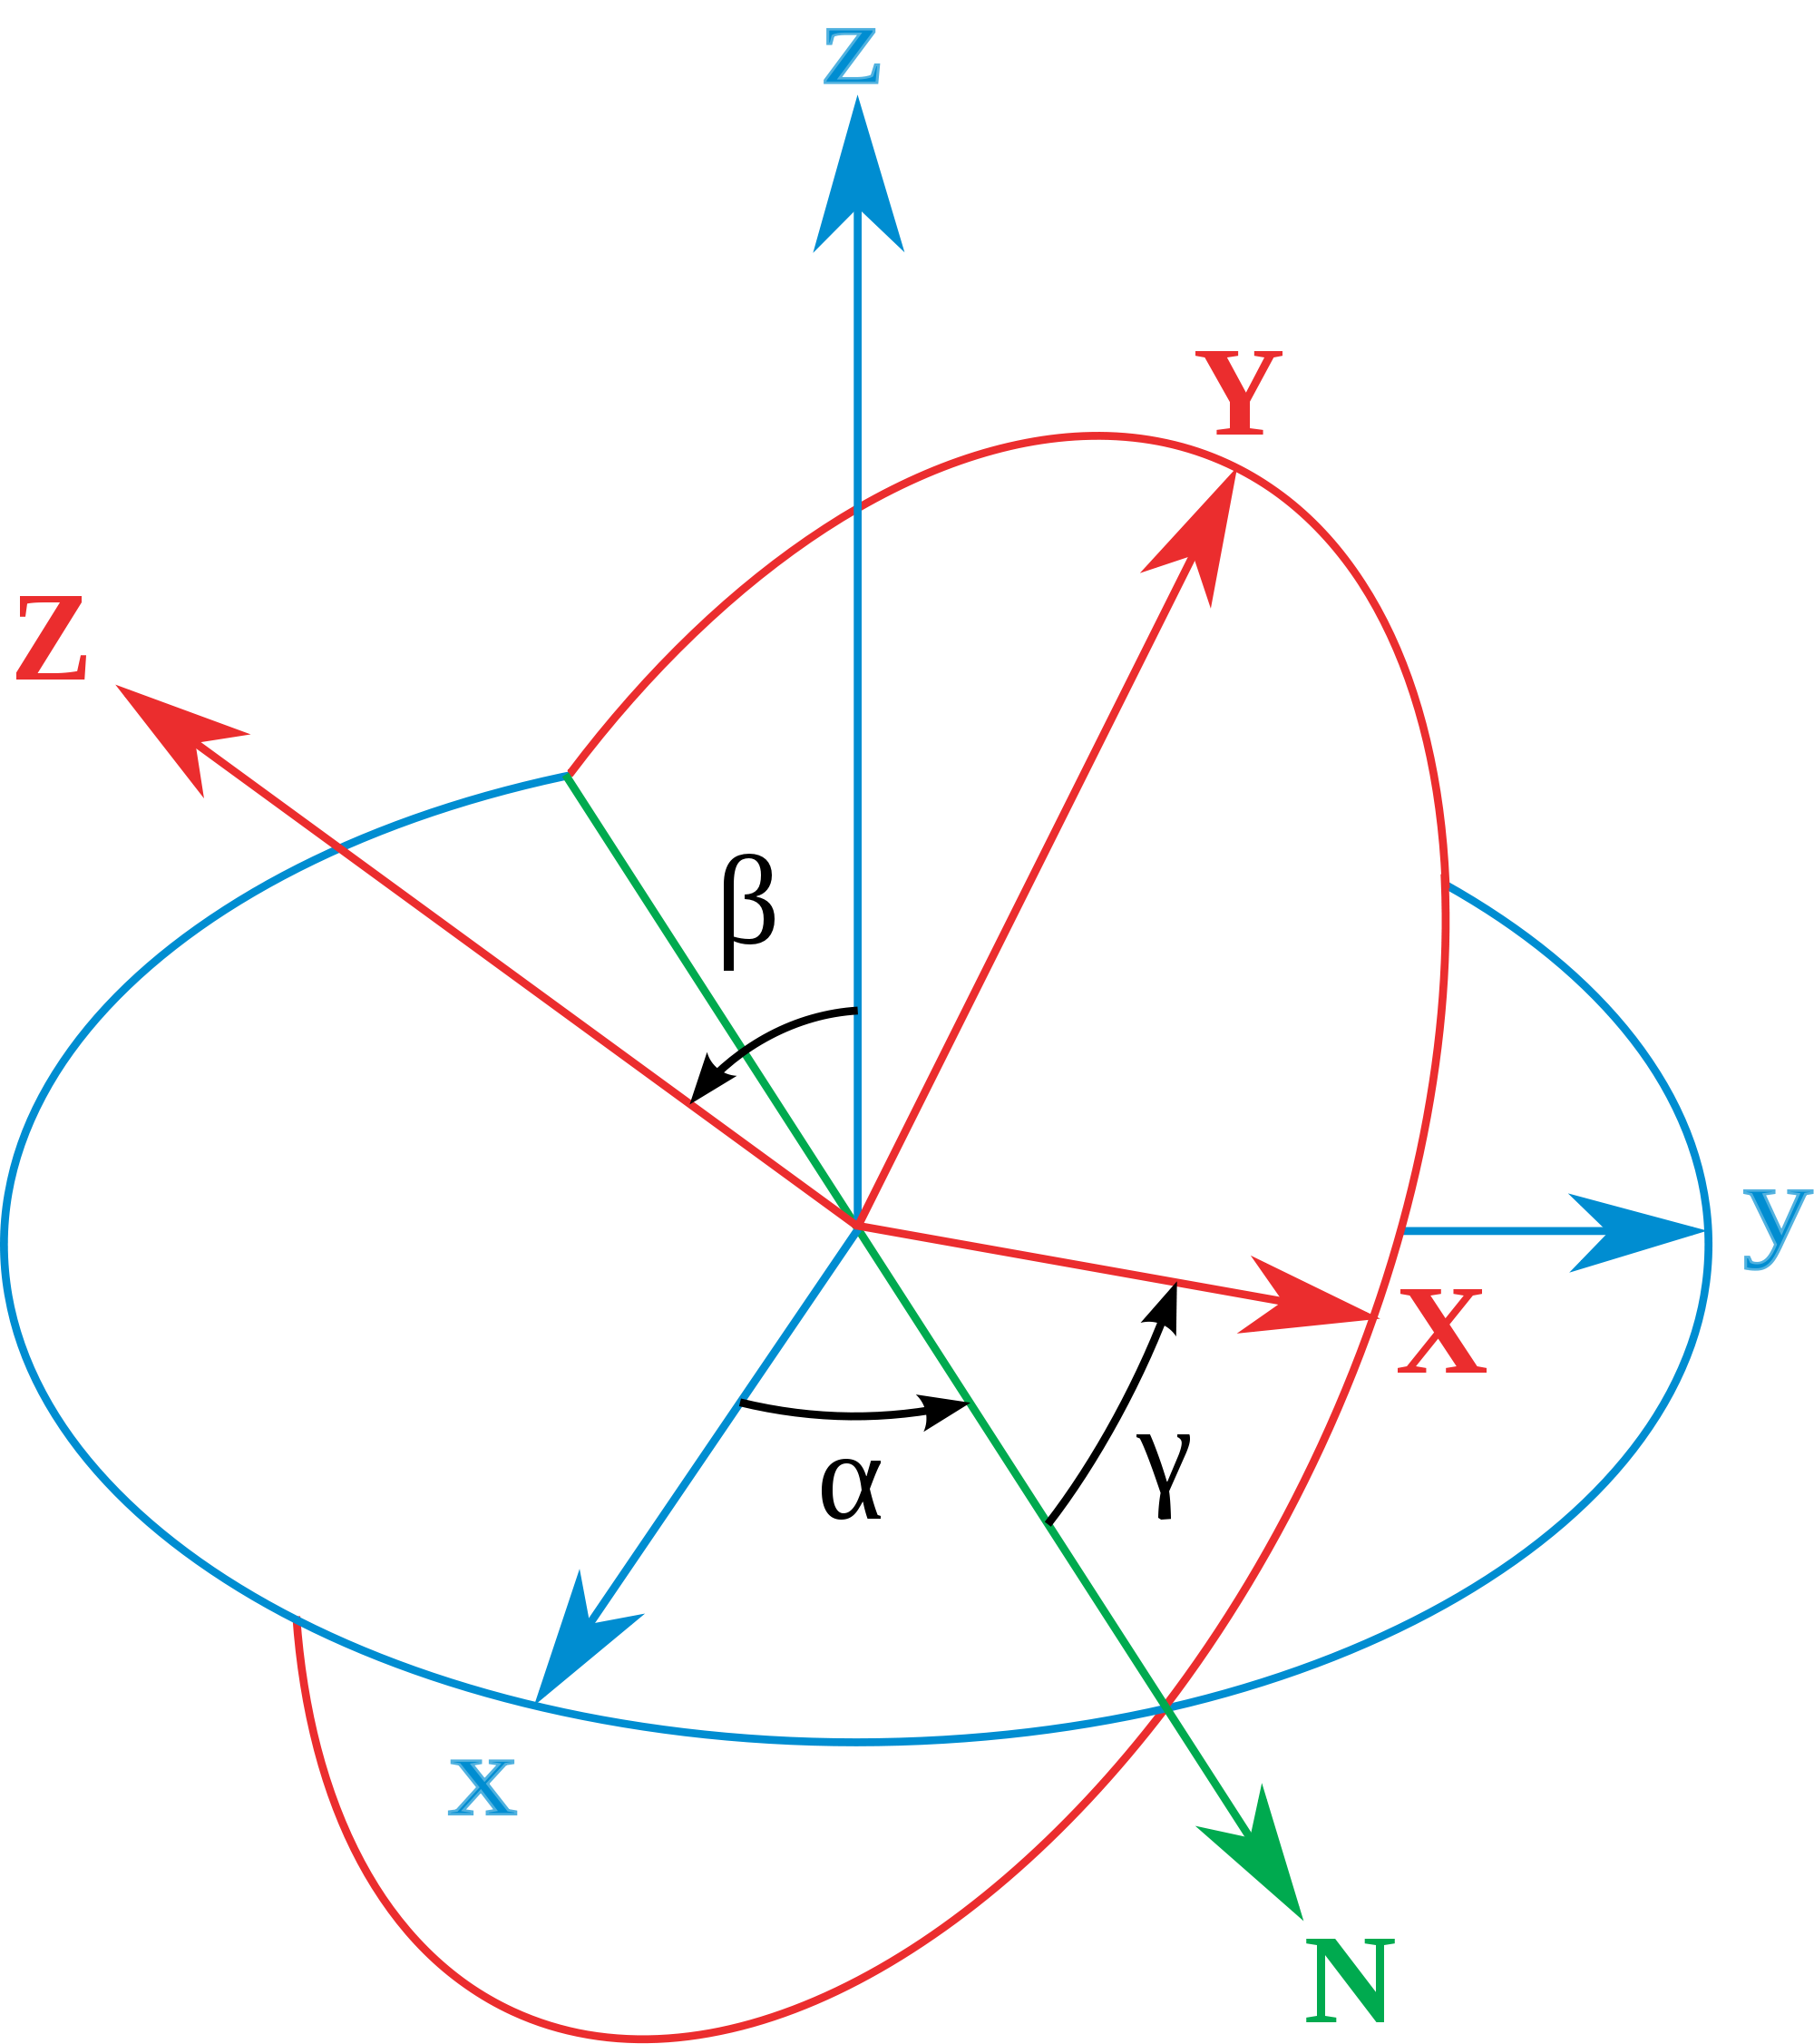
\includegraphics[scale=.05]{Euler_Angles.png}
\end{center}
where:
\begin{itemize}

\item
$(x,y,z)$ and $(X,Y,Z)$ represent the axes of the original and rotated frames

\item
$N$ is the intersection of the $xy$ and $XY$ planes

\item
$\alpha$ is the angle between the $x$ axis and the $N$ axis

\item
$\beta$ is the angle between the $z$ axis and the $Z$ axis

\item
$\gamma$ is the angle between the $N$ axis and the $X$ axis

\end{itemize}
The angles defined above are known as \textit{Proper Euler Angles} which provide us with:
\begin{itemize}

\item
A rotation about the $z$ axis that is determined by $\alpha$

\item
A rotation about the $N$ axis that is determined by $\beta$

\item
A rotation about the $Z$ axis that is determined by $\gamma$

\end{itemize}
\end{definition}
\end{minipage}}
\end{center}

\vspace{.3cm}
\section*{\underline{\textbf{Rotations}}}
\vspace{.3cm}
\begin{center}
\fbox{
\begin{minipage}{7.3 in}
\begin{definition}[Intrinsic Rotation] 
\textit{Intrinsic rotations} are ones that occur about the axes of the rotating coordinate system $XYZ$, keeping $xyz$ fixed. As a result the rotating coordinate system changes its orientation after each elemental rotation. 
\end{definition}
\end{minipage}}
\end{center}

\begin{example}
Begin by saying that the $XYZ$ coordinate system coincides with the $xyz$ system before we perform any rotation. Now let us say that we want to reach the final state above using intrinsic rotations. Follow these directions:
\begin{itemize}

\item
Rotate the $XYZ$ system by $\alpha$ about the $Z$ axis, which is the same as the $z$ axis.

\item
Rotate the new $XYZ$ system by $\beta$ about the new $X$ axis, which is the same as the $N$ axis above.

\item
Rotate the new $XYZ$ system by $\gamma$ about the new $Z$ axis, which is the $Z$ axis as in the image.

\end{itemize}
where this whole rotation would be written down as $Z-X'-Z''$ about the angles $\alpha$, $\beta$, and $\gamma$ respectively.
\end{example}

\vspace{.3cm}
\begin{center}
\fbox{
\begin{minipage}{7.3 in}
\begin{definition}[Intrinsic Rotation Matrix Form] 
An intrinsic rotation given by $X-Y'-Z''$ about the angles $\alpha$, $\beta$, and $\gamma$ respectively is given by:
\begin{equation*}
\mathcal{R} = X(\alpha)Y(\beta)Z(\gamma)
\end{equation*}
\end{definition}
\end{minipage}}
\end{center}

\vspace{.3cm}
\begin{center}
\fbox{
\begin{minipage}{7.3 in}
\begin{definition}[Extrinsic Rotation] 
\textit{Extrinsic rotations} are ones that occur about the axes of the fixed coordinate system $xyz$, keeping $xyz$ fixed.
\end{definition}
\end{minipage}}
\end{center}

\begin{example}
Begin by saying that the $XYZ$ coordinate system coincides with the $xyz$ system before we perform any rotation. Now let us say that we want to reach the final state above using extrinsic rotations. Follow these directions:
\begin{itemize}

\item
Rotate the $XYZ$ system by $\alpha$ about the $z$ axis.

\item
Rotate the new $XYZ$ system by $\beta$ about the $x$ axis.

\item
Rotate the new $XYZ$ system by $\gamma$ about the $z$ axis.

\end{itemize}
where this whole rotation would be written down as $z-x-z$ about the angles $\alpha$, $\beta$, and $\gamma$ respectively.
\end{example}

\vspace{.3cm}
\begin{center}
\fbox{
\begin{minipage}{7.3 in}
\begin{definition}[Extrinsic Rotation Matrix Form] 
An extrinsic rotation given by $x-y-z$ about the angles $\alpha$, $\beta$, and $\gamma$ respectively is given by:
\begin{equation*}
\mathcal{R} = Z(\gamma)Y(\beta)X(\alpha)
\end{equation*}
\end{definition}
\end{minipage}}
\end{center}

\begin{center}
\fbox{
\begin{minipage}{7.3 in}
\begin{definition}[Converting Between Extrinsic and Intrinsic] 
If we are given an extrinsic rotation $x-y-z$ about the angles $\alpha$, $\beta$, and $\gamma$ respectively:
\begin{equation*}
\mathcal{R} = Z(\gamma)Y(\beta)X(\alpha)
\end{equation*}
then this is equivalent to the intrinsic rotation $Z-Y'-X''$ about the angles $\gamma$, $\beta$, and $\alpha$ respectively.
\end{definition}
\end{minipage}}
\end{center}

\begin{center}
\fbox{
\begin{minipage}{7.3 in}
\begin{definition}[Gimbal Lock] 
A \textit{gimbal} is a ring that is suspended so it can rotate about an axis. Typically gimbals can be nested one within another to accommodate rotation about multiple axes such as:
\begin{center}
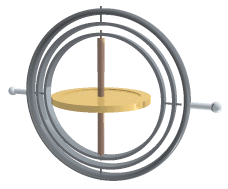
\includegraphics[scale=.5]{Gimbal.png}
\end{center}
\textit{Gimbal Lock} references the loss of one degree of freedom in a three dimensional, three-gimbal mechanism that occurs when the axes of two of the three gimbals are driven into a parallel configuration.
\end{definition}
\end{minipage}}
\end{center}

\begin{example}
Using Euler Angles, define the extrinsic rotation $z-y-x$ about the angles $\gamma$, $\beta$, and $\alpha$ respectively and observe what happens when $\beta = \frac{\pi}{2}$:
\begin{equation*}
\begin{split}
\mathcal{R} &= \begin{pmatrix}
1 & 0 & 0 \\
0 & \cos(\alpha) & -\sin(\alpha) \\
0 & \sin(\alpha) & \cos(\alpha)
\end{pmatrix} \begin{pmatrix}
\cos(\beta) & 0 & \sin(\beta) \\
0 & 1 & 0 \\
-\sin(\beta) & 1 & \cos(\beta)
\end{pmatrix} \begin{pmatrix}
\cos(\gamma) & -\sin(\gamma) & 0 \\
\sin(\gamma) & \cos(\gamma) & 0 \\
0 & 0 & 1
\end{pmatrix} \\
&= \begin{pmatrix}
1 & 0 & 0 \\
0 & \cos(\alpha) & -\sin(\alpha) \\
0 & \sin(\alpha) & \cos(\alpha)
\end{pmatrix} \begin{pmatrix}
0 & 0 & 1 \\
0 & 1 & 0 \\
-1 & 1 & 0
\end{pmatrix} \begin{pmatrix}
\cos(\gamma) & -\sin(\gamma) & 0 \\
\sin(\gamma) & \cos(\gamma) & 0 \\
0 & 0 & 1
\end{pmatrix} \\
&= \begin{pmatrix}
1 & 0 & 0 \\
0 & \cos(\alpha) & -\sin(\alpha) \\
0 & \sin(\alpha) & \cos(\alpha)
\end{pmatrix} \begin{pmatrix}
\cos(\gamma) & -\sin(\gamma) & 0 \\
\sin(\gamma) & \cos(\gamma) & 0 \\
0 & 0 & 1
\end{pmatrix} \\
&= \begin{pmatrix}
0 & 0 & 1 \\
\sin(\alpha)\cos(\gamma) + \cos(\alpha)\sin(\gamma) & -\sin(\alpha)\sin(\gamma) + \cos(\alpha)\cos(\gamma) & 0 \\
-\cos(\alpha)\cos(\gamma) + \sin(\alpha)\sin(\gamma) & \cos(\alpha)\sin(\gamma) + \sin(\alpha)\cos(\gamma) & 0
\end{pmatrix} \\
&= \begin{pmatrix}
0 & 0 & 1 \\
\sin(\alpha + \gamma) & \cos(\alpha + \gamma) & 0 \\
-\cos(\alpha + \gamma) & \sin(\alpha + \gamma) & 0
\end{pmatrix}
\end{split}
\end{equation*}
The final result ends up being a rotation that stays in the $z$ direction no matter what $\alpha$ and $\gamma$ are, thereby "locking" one of the directions.
\end{example}

\newpage
\begin{center}
\fbox{
\begin{minipage}{7.3 in}
\begin{proposition}[Useful Identity] 
Given any two vectors $u,v \in \mathbb{R}^3$, the following holds true:
\begin{equation*}
u \times v = u_{\times} v
\end{equation*}
where:
\begin{equation*}
u_{\times} = \begin{pmatrix}
0 & -u_3 & u_2 \\
u_3 & 0 & -u_1 \\
-u_2 & u_1 & 0
\end{pmatrix}
\end{equation*}
\end{proposition}
\end{minipage}}
\end{center}

\begin{proof}
This can be shown by direct computation of the determinant using the cofactor expansion and by reorganizing the linear result as the multiplication of a matrix and the vector on the right side:
\begin{equation*}
\begin{split}
u \times v &= \det\begin{pmatrix}
\hat{i} & \hat{j} & \hat{k} \\
u_1 & u_2 & u_3 \\
v_1 & v_2 & v_3 \\
\end{pmatrix} \\
&= \begin{pmatrix}
u_2v_3 - u_3v_2 \\
u_3v_1 - u_1v_3 \\
u_1v_2 - u_2v_1
\end{pmatrix} \\
&= \begin{pmatrix}
0 & -u_3 & u_2 \\
u_3 & 0 & -u_1 \\
-u_2 & u_1 & 0
\end{pmatrix} \begin{pmatrix}
v_1 \\
v_2 \\
v_3
\end{pmatrix}
\end{split}
\end{equation*}
\end{proof}

\begin{center}
\fbox{
\begin{minipage}{7.3 in}
\begin{proposition}[Rotation Matrix for Rotation About Any Axis] 
A rotation about a given a unit vector $\hat{k} \in \mathbb{R}^3$ with angle $\theta$ is determined by the rotation matrix:
\begin{equation*}
\mathcal{R} = \begin{pmatrix}
\cos(\theta)(1 - k_1^2) + k_1^2 & k_1k_1(1 - \cos(\theta)) - k_3\sin(\theta) & k_1k_3(1 - \cos(\theta)) + k_2\sin(\theta) \\
k_1k_2(1 - \cos(\theta)) + k_3\sin(\theta) & \cos(\theta)(1 - k_2^2) + k_2^2 & k_2k_3(1 - \cos(\theta)) - k_1\sin(\theta) \\
k_1k_3(1 - \cos(\theta)) - k_2\sin(\theta) & k_2k_3(1 - \cos(\theta)) + k_1\sin(\theta) & \cos(\theta)(1 - k_3^2) + k_3^2
\end{pmatrix}
\end{equation*}
\end{proposition}
\end{minipage}}
\end{center}

\begin{proof}
If we accept Rodrigues' Rotation Formula:
\begin{equation*}
v' = \cos(\theta)v + \sin(\theta)(\hat{k} \times v) + (1 - \cos(\theta))\hat{k}(\hat{k} \cdot v)
\end{equation*}
then if we simply pull out the vector on the right side and combine we get:
\begin{equation*}
\begin{split}
v' &= \cos(\theta)v + \sin(\theta)\hat{k}_{\times}v + (1 - \cos(\theta))\hat{k}\hat{k}^T v \\
&= \Big[ \cos(\theta)I_3 + \sin(\theta)\hat{k}_{\times} + (1 - \cos(\theta))\hat{k} \otimes \hat{k} \Big] v \\
&= \Bigg[ \begin{pmatrix}
\cos(\theta) & 0 & 0 \\
0 & \cos(\theta) & 0 \\
0 & 0 & \cos(\theta)
\end{pmatrix} + \begin{pmatrix}
0 & -k_3\sin(\theta) & k_2\sin(\theta) \\
k_3\sin(\theta) & 0 & -k_1\sin(\theta) \\
-k_2\sin(\theta) & k_1\sin(\theta) & 0
\end{pmatrix} \\
& \hspace{.4cm} + (1 - \cos(\theta))\begin{pmatrix}
k_1^2 & k_1k_2 & k_1k_3 \\
k_1k_2 & k_2^2 & k_2k_3 \\
k_1k_3 & k_2k_3 & k_3^2
\end{pmatrix} \Bigg] v \\
&= \begin{pmatrix}
\cos(\theta)(1 - k_1^2) + k_1^2 & k_1k_1(1 - \cos(\theta)) - k_3\sin(\theta) & k_1k_3(1 - \cos(\theta)) + k_2\sin(\theta) \\
k_1k_2(1 - \cos(\theta)) + k_3\sin(\theta) & \cos(\theta)(1 - k_2^2) + k_2^2 & k_2k_3(1 - \cos(\theta)) - k_1\sin(\theta) \\
k_1k_3(1 - \cos(\theta)) - k_2\sin(\theta) & k_2k_3(1 - \cos(\theta)) + k_1\sin(\theta) & \cos(\theta)(1 - k_3^2) + k_3^2
\end{pmatrix} v
\end{split}
\end{equation*}
\end{proof}




\end{document}